\chapter{Diodes and How to Use Them}
\label{chapDiodes}

% FIXME - make sure I talk about safety concerns and reference the power chapter.

This chapter introduces the \glossterm{diode}.  
We have used light-emitting diodes (LEDs) in previous chapters, but have not really discussed their function except for emitting light.
In this chapter, we are going to look at regular diodes, light-emitting diodes, and Zener diodes, to get a feel for what these devices are and how they might be used in circuits for more than just light.

% FIXME - schematic of a diode

\section{Basic Diode Behavior}

Unlike resistors, diodes have both a positive and negative side.
For any component with both positive and negative legs, the positive leg of the component is termed the \glossterm{anode} and the negative leg is termed the \glossterm{cathode}.
On LEDs, the anode is longer than the cathode.
However, for other types of diodes, the cathode is marked with a line.
You can remember this because in the schematic of a diode, the cathode has the blocking line.

The diode performs two fundamental ``actions'' with electric current.  
The first action of a diode is to drop voltage by an essentially fixed amount \emph{without} affecting or limiting current.
This amount of voltage is called the \glossterm{forward voltage drop} and it is usually around $0.6\myvolt$ for more non-LED diodes. 
Forward voltage is often abbreviated as $\myvolt_F$.
For most LEDs, the forward voltage drop depends on the color of the LED, with a red LED dropping about $1.8\myvolt$ and a blue LED dropping about $3.3\myvolt$.
The forward voltage drop can vary among the other colors as well.

To remind you, when we say ``voltage drop,'' we are referrig to the difference in voltage between the positive and negative leg of the diode.
Therefore, no matter what the voltage is coming into the diode, the voltage coming out of the diode will be that voltage minus the voltage drop.

The second action of a diode is to limit the direction of current to a single direction.
With some exception, the diode only allows current to flow one way in the circuit.
The ``normal flow'' of a current through the diode is to flow from the anode to the cathode.
Looking at the schematic symbol, current flows in the direction that the arrow is pointing, and current is blocked from flowing the other way (you can think of the line as a ``block'' preventing reverse flow).

However, diodes are limited in the amount of reverse flow they can block.
At a certain point, diodes reach their \glossterm{breakdown voltage}.
The breakdown voltage is the voltage at which they will stop blocking voltage.
In regular diodes, this is a failure mode and the precise value shouldn't be relied upon (we will see an exception to this with Zener diodes). %% FIXME - refer to specific section on Zener diodes
Usually, though, this value is high enough not to worry about (i.e., around 100 volts).

\section{Circuit Calculations with Diodes in Series}

Now let's talk about how to properly calculate the behavior of circuits with diodes.
Remember, the key to a diode is that if current is flowing through the diode, the voltage drop across the diode will be essentially constant.
For a normal non-LED diode, this voltage drop is almost always $0.6\myvolt$.
This is so common it is usually assumed, and never listed in the circuit itself.

Therefore, take a look at the circuit in Figure~\ref{figDiodeWithResistor}.
Since the voltage source is 9 volts, that means that the total voltage drop between the positive and negative is 9 volts.
The diode will eat $0.6\myvolt$ of the voltage, but will not limit the current in any way.
The resistor, then, since it is the only component left, will use up the rest of the voltage---$8.4\myvolt$.
Therefore, we can calculate the current in the circuit using Ohm's law:

$$I = V / R = 8.4 / 1000 = 0.0084\myamp = 8.4\mymamp$$

\simplegraphicsfigure{A Diode and Single Resistor Circuit}{DiodeWithResistor}{0.08}

Therefore, our circuit will use $8.4\mymamp$ of current.
So, as you can see, when doing calculations, the diodes simply provide a drop in voltage, they do not limit current.

This is true no matter how many diodes or resistors I have in my circuit.
Figure~\ref{figMultipleDiodesResistors} shows a circuit like that.
To figure out the behavior of this circuit, remember that \emph{every} diode has a $0.6\myvolt$ voltage drop.  Since the circuit has three diodes, that means that the diodes will drop a total of $0.6 * 3 = 1.8\myvolt$.

Therefore, we will have $1.8\myvolt$ taken up by diodes, which drop voltage without limiting current.  
Since we have a $9\myvolt$ source, there will be $9 - 1.8 = 7.2\myvolt$ that is not eaten by diodes.
This voltage will go to our two resistors.  
These resistors, even though they are separated by diodes, are essentially in series with each other.
Therefore, we can treat them as a single resistor in series.
So, the total resistance on the circuit will be $1k + 2k = 3k\myohm$.

We can then find the total current running through the circuit using Ohm's Law:

$$ I = V / R = 7.2\myvolt / 3,000\myohm = 0.0024\myamp = 2.4\mymamp$$

\simplegraphicsfigure{A Circuit with Multiple Diodes and Resistors}{MultipleDiodesResistors}{0.08}

However, it is possible to put too many diodes in your circuit.
Since they each eat $0.6\myvolt$ in their forward voltage drop, that puts a limit on how many you can string together in series from a given battery.
For a $9\myvolt$ battery, if I try to put 20 diodes together in series, I will have used \emph{more} than the total 9 volts that I have available.  
Therefore, current will not flow.
With 20 diodes, the voltage drop will be $20 * 0.6 = 12\myvolt$.  
Since this is more voltage than the battery can put out, no current will flow.

So, we have seen two conditions for which current will not flow through a diode---the first is that the diode will block current from flowing in the wrong direction, and the second is that the diode will not conduct if the voltage source cannot provide enough voltage to bridge the forward voltage drop of the diode.

\section{Circuit Calculations with Diodes in Parallel}

The real magic of diodes comes when using them in parallel circuits.
Remember the rules that we learned in Chapter~\ref{chSeriesParallel}.
Kirchoff's Voltage Law says that between any two points, the voltage drop between those two points will be the same \emph{no matter what path the current follows}.
Therefore, since the voltage drop across a diode is \emph{fixed}, that means that we can guarantee a maximum voltage drop between two points on a circuit by putting diodes between them.

\simplegraphicsfigure{A Single Diode in Parallel with a Resistor}{ParallelDiode}{0.08}

Figure~\ref{figParallelDiode} shows what this looks like.  
The voltage drop from one side of the diode to the other is $0.6\myvolt$.
Period. End of story (actually, it could be less, which would keep the diode from conducting altogether, but we won't consider that at the moment).

Kirchoff's Voltage Law tells us that \emph{no matter what path is travelled}, the voltage difference between those two points will be the same.
Since the 2k resitor is attached to the same two points that the diodes are attached to, Kirchoff's Voltage Law tells us that the voltage across the resistor \emph{must} be the same as the voltage across the diode.
Thus, the voltage across the resistor \emph{must} be $0.6\myvolt$.

Using Ohm's law, we can deduce the amount of current flowing through that resistor:

$$ I = V / R = 0.6 / 2,000 = 0.0003\myamp = 0.3\mymamp $$

So how much current is flowing through the diode?
To find this out, we need to use Kirchoff's Current Law.
The amount entering the junction where the diode and the 2k resistor splits off is the same as the amount leaving it.
We know that $0.3\mymamp$ leaves the junction to go to the resistor.
Therefore, if we could figure out how much current was coming \emph{into} the junction we could figure out how much is going through the diode.

To discover that value, we need to know how much current is going through the 1k resistor.
To figure that out, we need to know the voltage drop across the resistor.
However, we can figure this out easily.  
Since the tail end of the diode is connected to ground (the negative terminal), that means that after the diode we are at $0\myvolt$.  
Therefore, since the diode voltage drop is $0.6\myvolt$, then the voltage before the diode must be $0.6\myvolt$.
That means that the rest of the voltage must have been consumed by the 1k resistor.

Since the voltage source is $9\myvolt$, that means that the voltage for the entire circuit from positive to negative is $9\myvolt$, and therefore, the voltage drop across the resistor must have been $9 - 0.6 = 8.4\myvolt$.
Using this value, we can determine the current going through the resistor using Ohm's Law.

$$ I = V / R = 8.4 / 1,000 = 0.0084\myamp = 8.4\mymamp $$

In this circuit, there is $8.4\mymamp$ going through the first resistor.
That means that there is $8.4\mymamp$ coming into the junction.
We know that $0.3\mymamp$ is going out of the junction through the 2k resistor.
That means that the rest of the current is going through the diode.
Therefore, we can calculate that the current going through the diode is $8.4 - 0.3 = 8.1\mymamp$.

Diodes don't make the math harder, but they do force you to think a little harder about how you apply the rules.

Let's take a look at a slightly harder example, using Figure~\ref{figParallelMultipleDiodes}.
In this circuit, we have two diodes in parallel with two resistors in parallel.
This parallel circuit is in series with a resistor on the front and another diode at the end. 

\simplegraphicsfigure{A Circuit with Multiple Diodes}{ParallelMultipleDiodes}{0.08}

It is almost always easiest to analyze circuits starting with the diodes because their voltage drops are fixed.
If we look at this circuit, the diode at the end gives the circuit a voltage drop of $0.6\myvolt$.

Now let's look at the parallel part of the circuit.
Here, we have three pathways---one through two diodes, and two other pathways through resistors.
However, one of the pathways contains all diodes.
We know that diodes give a constant voltage drop, and we know that Kirchoff's Voltage Law says that all pathways between two points have the same voltage drop.
Since we have two diodes, the voltage drop of this parallel pathway is $0.6 * 2 = 1.2\myvolt$.

Now we have the parallel resistors to worry about.
However, we can use the formula for parallel resistance (Equation~\ref{eqparallelresistancen}) to figure out the total resistance of the parallel resistors.

$$ R_T = \frac{1}{\frac{1}{R1} + \frac{1}{R2}} = \frac{1}{\frac{1}{2,000} + \frac{1}{3,000}} \approx \frac{1}{0.0005 + 0.0003333} = \frac{1}{0.0008333} \approx 1200\myohm $$

However, we technically don't even need that number, because, since we already know the voltage drop across each resistor (it \emph{must} be $1.2\myvolt$ because of Kirchoff's Voltage Law), we can just apply Ohm's Law to each resistor.

Now, using Ohm's Law, we can calculate the current flowing through the resistors.
So, for the 2k resistor, we have:

$$ I = V / R = 1.2\myvolt / 2,000\myohm = 0.0006\myamp = 0.6\mymamp $$

For the 3k resistor, we have:

$$ I = V / R = 1.2\myvolt / 3,000\myohm = 0.0004\myamp = 0.4\mymamp $$

The total current going into both resistors is simple the sum of each of the currents, $0.4 + 0.6 = 1.0\mymamp$.
So there is $1\mymamp$ total flowing through the two resistors.
To find out how much current is flowing through the diode, we will need to know how much current is coming into the circuit itself out of the first resistor.

So how much current is flowing through the first resistor?
Well, the voltage drops we have calculated so far include a $0.6\myvolt$ drop at the end and a $1.2\myvolt$ drop in the middle.
That is a total of $1.2 + 0.6 = 1.8\myvolt$.
Since the battery is $9\myvolt$, that means that there is $9 - 1.8 = 7.2\myvolt$ left to be consumed by the circuit.
Therefore, that must be the voltage drop of the first resistor.
Using Ohm's Law, we find that:

$$ I = V / R = 7.2\myvolt / 1,000\myohm = 0.0072\myamp = 7.2\mymamp $$

Therefore, we have $7.2\mymamp$ flowing through that first resistor.
So, if we have $7.2\mymamp$ coming into the parallel circuit in the middle, and $1\mymamp$ flowing to the resistors, the amount of current flowing through the diodes down the middle is $7.2 - 1 = 6.2\mymamp$.
The amount of current going through the final diode is the full $7.2\mymamp$ of current in the circuit.

Again, there are a lot of steps, but none of the steps are individually very hard.
You simply start with the easiest-to-find values (in this case, the voltage drops from the diodes), and work out from there.

\section{Diode Short Circuits}

Next, let's look at a very bad design with a diode.
Let's say that someone wanted to use a diode to regulate the amount of voltage across a resistor to $0.6\myvolt$.
Therefore, they built the circuit shown in Figure~\ref{figBadDiodeCircuit}.
Can you figure out what the problem is here?

\simplegraphicsfigure{A Bad Diode Circuit}{BadDiodeCircuit}{0.08}

Well, the voltage drop across the diode will be $0.6\myvolt$.
However, the battery operates at $9\myvolt$.  
This means that there is $8.4\myvolt$ left in the circuit with \emph{zero} resistance.
Using Ohm's Law, that gives us:

$$ I = V / R = 8.4 / 0 = \infty $$

Thus, having a diode going direct from the positive to the negative of your voltage source is essentially the same as a short circuit.  
That is why the circuit is bad!
To use a diode, there must \emph{always} be resistance somewhere in series with the diode whether the resistance comes before it or after it in order to dissipate the current from the excess voltage.

\section{Non-Conducting Diodes}

There is one case where diodes do not maintain a constant voltage drop, and that is where there is not enough voltage to go across them.
Figure~\ref{figNonconductingDiodes} shows an example of this.

\simplegraphicsfigure{Nonconducting Diodes}{NonconductingDiodes}{0.08}

In this figure, the voltage drop across the center diode bridge is $0.6 + 0.6 + 0.6 + 0.6 = 2.4\myvolt$.
However, the battery source is only $1\myvolt$.
Since the voltage drop of the diodes is larger than the available voltage, this part of the circuit is basically turned off.
In reality, there is a small but ignorable leakage current (about $0.00000022\mymamp$ in this case), but we can think of this circuit as effectively switched off.

So keep that in mind---if you ever wind up with more forward voltage drop from a diode than you have available voltage, you may treat the diode as if it were an open (i.e., unconnected) circuit---as if it were not even there.

Therefore, we would analyze Figure~\ref{figNonconductingDiodes} as if it were just like Figure~\ref{figNonconductingDiodesNoDiodes}.

\simplegraphicsfigure{A Circuit Equivalent to Figure~\ref{figNonconductingDiodes} Because of Nonconducting Diodes}{NonconductingDiodesNoDiodes}{0.08}

\section{Usage of Diodes}

Diodes can be thought of as circuit traffic cops---they regulate the flow of electricity.
They make sure that everything within a circuit is happening in a controlled manner.
They regulate the circuit in two different ways---both by limiting the direction of current and, in parallel circuits, by establishing fixed voltages between two points.

The simplest usage of a diode is to use it as a device that makes sure that your battery is in the right direction.
If you have a device that will be damaged if someone puts the battery in backwards, a simple diode will make sure that the current can only flow in one direction.

\simplegraphicsfigure{A Simple Diode Protection Circuit}{SimpleDiodeCircuit}{0.08}

The circuit in Figure~\ref{figSimpleDiodeCircuit} shows what this looks like.
Note that we have a resistor labelled ``load.''  
Many times in circuits, a load resistor is shown to represent whatever else is happening in another part of a circuit.
Thus, this circuit shows that the diode is protecting the rest of the circuit (whatever it is) from the user putting the battery in backwards.
However, this has a cost---the diode will eat $0.6\myvolt$ in order to provide this protection.

Another problem often solved by diodes is voltage regulation.
Because diodes provide a fixed voltage drop between two points, you can use diodes to ensure a fixed voltage for devices that require it.

For instance, when we looked at batteries in Chapter~\ref{chapConstructingTesting}, we noted that their voltage actually varied quite a bit.
A $9\myvolt$ battery might give you anywhere from $7\myvolt$ to $9.7\myvolt$.
This is true of any battery, not just the $9\myvolt$ variety.

Therefore, if you need a fixed amount of voltage, you can use diodes to provide that at the cost of some extra current.

Figure~\ref{figThreeVoltDiodeRegulator} shows a simple voltage regulator using diodes.
Given a $5\myvolt$ battery (actually, a battery of any size significantly over $3\myvolt$ will work), this circuit will provide a regulated $3\myvolt$ of electricity to whatever is connected to it as a load (remember, a ``load'' resistor is just a stand-in for whatever we want to attach to this).

\simplegraphicsfigure{A Simple $3\myvolt$ Voltage Regulator}{ThreeVoltDiodeRegulator}{0.08}

Because the diodes provide a fixed voltage drop of $0.6\myvolt$ each, then that pathway has a total voltage drop for five diodes as $5 * 0.6 = 3.0\myvolt$.
Kirchoff's Voltage Law says that between two points, \emph{every} pathway between them will have the same voltage drop.
This means that the load, since it is connected to those two points, will have the same voltage drop, thus regulating the amount of voltage used by the load.

But what about that first resistor at the beginning of the circuit?
Remember, if we provide a pathway through diodes only, we create a short circuit in the system.
There has to be some element (usually a resistor) that eats up whatever voltage is left over.
Therefore, putting a small resistor before our diode pathway will give the circuit a place to use the excess voltage, and limit the amount of current that flows.

The size of the resistor will depend on how much current the load requires and how much current you are willing to waste.
A small resistor wastes more current, but allows for a higher maximum current used by the load.
A larger resistor wastes less current, but if the load needs a lot of current, it could interfere with the voltage regulation.

To see how this could happen, let's say that our load is equivalent to $1,000\myohm$.
This means that the amount of current that the load will draw can be calculated using Ohm's Law:

$$ I = V / R = 3\myvolt / 1,000\myohm = 0.003\myamp = 3\mymamp $$

So the load will use up $3\mymamp$ of current.
That means that, however much current goes through our first resistor, however much that is over $3\mymamp$ will be drained off through the diodes.
So, let's calculate what that looks like on a tiny, $20\myohm$ resistor.
The voltage will be $5 - 3 = 2\myvolt$.

$$ I = V / R = 2\myvolt / 20\myohm = 0.1\myamp = 100\mymamp $$

So, if we just used a $20\myohm$ resistor, that means that even though the load only used $3\mymamp$, the whole circuit will be using $100\mymamp$ to operate!
Therefore, we need a bigger resistor to limit the amount of current we use.
Let's try a $500\myohm$ resistor:

$$ I = V / R = 2\myvolt / 500\myohm = 0.004\myamp = 4\mymamp $$

This is much better---we are only using $4\mymamp$ in this circuit, so we are only wasting $1\mymamp$.
There has to be \emph{some} amount of waste to do the voltage regulation.

Let's say that, after a while, our battery sags down to only providing $4\myvolt$ of power.
What happens now?
Well, using the $500\myohm$ initial resistor, that means that there is only $1\myvolt$ extra to drain off, so the current will be:

$$ I = V / R = 1\myvolt / 500\myohm = 0.002\myamp = 2\mymamp $$

Here, the current is only $2\mymamp$, but we need $3\mymamp$ to power the circuit!
Thus, if we use a $500\myohm$ resistor, we can't handle our power supply dropping down to $4\myvolt$.

What about using the $20\myohm$ resistor?
In this case, Ohm's Law would give us:

$$ I = V / R = 1\myvolt / 20\myohm = 0.05\myamp = 50\mymamp $$

So, here, the $20\myohm$ resistor will still provide plenty of excess current to allow our regulator to keep working.
However, it is still eating up an extraordinary amount of current compared to our load.

So how do you choose the right resistor?
The way to work situations like this is to think about what are the maximum cases you are designing for, and then calculate appropriately.
So, if I want this circuit to work when the battery sags down to $4\myvolt$, I need to decide how much excess current I'm willing to have at that level.
Let's say I decide that I always want at least half a milliamp to run through the diode (somewhat of an arbitrary number, but if the diode has no power, it is not providing any regulation---this is a low number that is still ``noticeable'' on the circuit).
That means that, since my load will be using $3\mymamp$, the total amount of current running through the initial resistor will be $3.5\mymamp$, or $0.0035\myamp$.
Therefore, I calculate what the resistor will need to be a $4\myvolt$ using Ohm's Law:

$$ R = V / I = 1\myvolt / 0.0035\myamp \approx 286\myohm $$

Therefore, for this situation, the initial resistor should be $286\myohm$.
Now, let's figure out how much current this wastes when the battery is at full charge---$5\myvolt$ (which means that there will be a $2\myvolt$ drop across this resistor).

$$ I = V / R = 2\myvolt / 286\myohm \approx 0.007\myamp = 7\mymamp $$

So, at full charge, there is $7\mymamp$ going through this resistor, which means we will waste $4\mymamp$.  
Whether or not that is acceptable to your circuit depends on what you are going to do with it!

Note that there are better means of regulating battery voltage for a whole circuit than using diodes.
However, many times you need a regulated voltage somewhere \emph{within} a more complex circuit.
Diodes are great for that, and the same calculations apply.

One final note---as mentioned earlier, although we think of diodes as providing a fixed voltage, they actually do vary a little bit with the amount of current flowing through them.
In any circuit, you should allow for $\pm 10\%$ variance in the voltage drop of a diode.

\section{Other Types of Diode Protection}

Diodes can provide other types of protection for circuits as well.
As single-direction control valves, they can be used to prevent a variety of over-voltage conditions.
Often times they are wired in such a way that they will not normally conduct, but will conduct under certain conditions to redirect extra voltage in a safe manner.

Figure~\ref{figFlybackDiode} shows an example circuit.
In this circuit, a DC motor is connected to a switch.
Notice the diode that is wired backwards.
Normally, this diode does absolutely nothing because the current is flowing in the other direction, so it just goes through the motor.
DC motors, however, tend to generate very large voltages for a short time when switched off.
Therefore, when this motor is switched off the motor can produce a very large voltage---up to $50\myvolt$ in this circuit!

\simplegraphicsfigure{A Diode Protection Circuit}{FlybackDiode}{0.08}

To protect the rest of the circuit from this sudden influx of voltage, the diode provides an alternative path back through the motor.
Thus, when the voltage starts to build up after the switch closes, the diode provides a safe pathway back through motor for it to flow, allowing the voltage buildup to slowly dissipate through the motor, rather than overloading a circuit expecting $5\myvolt$ with $50\myvolt$.

Often times when looking at circuit diagrams you may find diodes in funny places, and oriented in funny ways.
These are oftentimes providing some sort of protection to the circuit from potential failure conditions or exceptional circumstances.
Many microchips, for instance, use diodes to shunt off excess voltage from static electricity shocks.

\section{Zener Diodes}

One problem with using diodes for voltage regulation is that their forward voltage drop is pretty small, so you have to have quite a few of them to regulate larger voltages.
Zener diodes can help out in these situations.
Figure~\ref{figZenerDiodeSymbol} shows the symbol for a Zener diode.

\simplegraphicsfigure{The Zener Diode Schematic Symbol}{ZenerDiodeSymbol}{0.08}

Remember that most diodes have a breakdown voltage if you try to pass voltage the wrong way.
However, in most diodes, this is a failure mode---doing this can, at best, be unpredictable, and, at worst, damage your diode.
A Zener diode, however, is built so that it has a very predictable operation at its breakdown voltage.
In fact, at its breakdown voltage, it acts like a normal diode with a larger voltage drop.

However, since you are using the breakdown voltage rather than the forward voltage, Zener diodes are wired into your circuit \emph{backwards}.
Figure~\ref{figZenerAndRegular} shows what this looks like.
In this figure, on the left you have the same $3\myvolt$ regulated circuit as above.
On the right, you have an equivalent circuit regulated by a Zener diode instead.
Since we are using the Zener diode's breakdown voltage rather than its forward voltage, it has to be wired backwards for it to work.

\simplegraphicsfigure{A Circuit Regulated by Regular Diodes and a Zener Diode}{ZenerAndRegular}{0.08}

Not only that, the breakdown voltage drop for a Zener diode is much more constant over a larger range of current than the forward voltage drop of most regular diodes.
Because of this, Zener diodes are used much more often for voltage regulation than series of regular diodes.

Zener diodes come in a variety of breakdown voltages.  
In any exercise in this book which involves drawing a circuit with a Zener diode, you may presume that the Zener diode with the voltage drop you are looking for exists.
When drawing a circuit, be sure to label the Zener diode with the breakdown voltage you are needing.

\reviewsection

In this chapter, we learned:

\begin{enumerate}
\item Diodes only allow current to flow in one direction.
\item Diodes have a fixed forward voltage drop across the diode---$0.6\myvolt$ for normal diodes, and a range of about $1.8--3.3\myvolt$ for LEDs.
\item Different color LEDs have different voltage drops.
\item Diodes also have a breakdown voltage---the amount of voltage for which, if applied in the reverse direction, the diode will no longer block current.
\item When analyzing circuits with diodes, it is often easier to analyze the diodes first, since the voltage drop is fixed.  
\item Because of Kirchoff's Voltage Law, anything wired in parallel with diodes will have the same voltage drop as the diodes.
\item If the forward voltage drop on a diode is greater than the available voltage in the circuit, the diode will not conduct and it can be treated as an open circuit.
\item If diode(s) are connected to the positive and negative terminals of a voltage source (such as a battery) with no resistance in series, this will create a short circuit, causing extremely large amounts of current to flow through the diode.
\item Diodes are often used to regulate the amount of voltage between two points on a circuit.
\item Diodes are often used as control valves to regulate the direction of current flow on a circuit.
\item Diodes can be used as voltage regulators to provide a predictable amount of voltage to a circuit with changing battery conditions.
\item The series resistor used with voltage-regulating diodes determines both how much current is wasted and how much current the load can draw---lower-value resistors waste more current but allow the load to draw more current, and higher-value resistors waste less current but don't allow as much potential current to your load.
\item When designing circuits, it is often useful to account for the most extreme variations possible.  This will allow your circuit to be more flexible.
\item Diodes can also provide protection to circuits against strange failure conditions, such as voltage spikes and static electricity.  Diodes in strange places in circuit diagrams are often there to protect the circuit against certain types of failures or events.
\item Zener diodes are built so that they have very reliable operation on their breakdown voltage.  
\item Wiring a Zener diode backwards gives you the equivalent of several forward diodes in series, and can be used for simple voltage regulation.
\item The breakdown voltage of a Zener diode is much more constant than the forward voltage of a regular diode, and therefore works even better for voltage regulation.
\item Zener diodes come in a wide variety of breakdown voltages and are usually labelled on the circuit with the necessary breakdown voltage.
\end{enumerate}

\applysection


\begin{enumerate}
\item If you have a $9\myvolt$ voltage source, a blue LED, and a $500\myohm$ resistor all in series, how much current is running through the LED?
\item If you have a $3\myvolt$ voltage source and a red LED, what size resistor do you need to put in series with the LED to have it use $3\mymamp$ of current?
\item If you have a $10\myvolt$ voltage source, a blue LED, a red LED, and a $200\myohm$ resistor all in series, how much current is running through the LEDs?
\item If I have a $12\myvolt$ voltage source, a blue LED, and a red LED, and the LEDs have a maximum current of $30\mymamp$ before it breaks and a minimum current of $1\mymamp$ before it turns on, what range of resistors can I put in series with the LEDs to get them to light up without breaking?
\item In the circuit below, calculate the how much current flowing through each component and each component's voltage drop if R1 is $500\myohm$. \\ 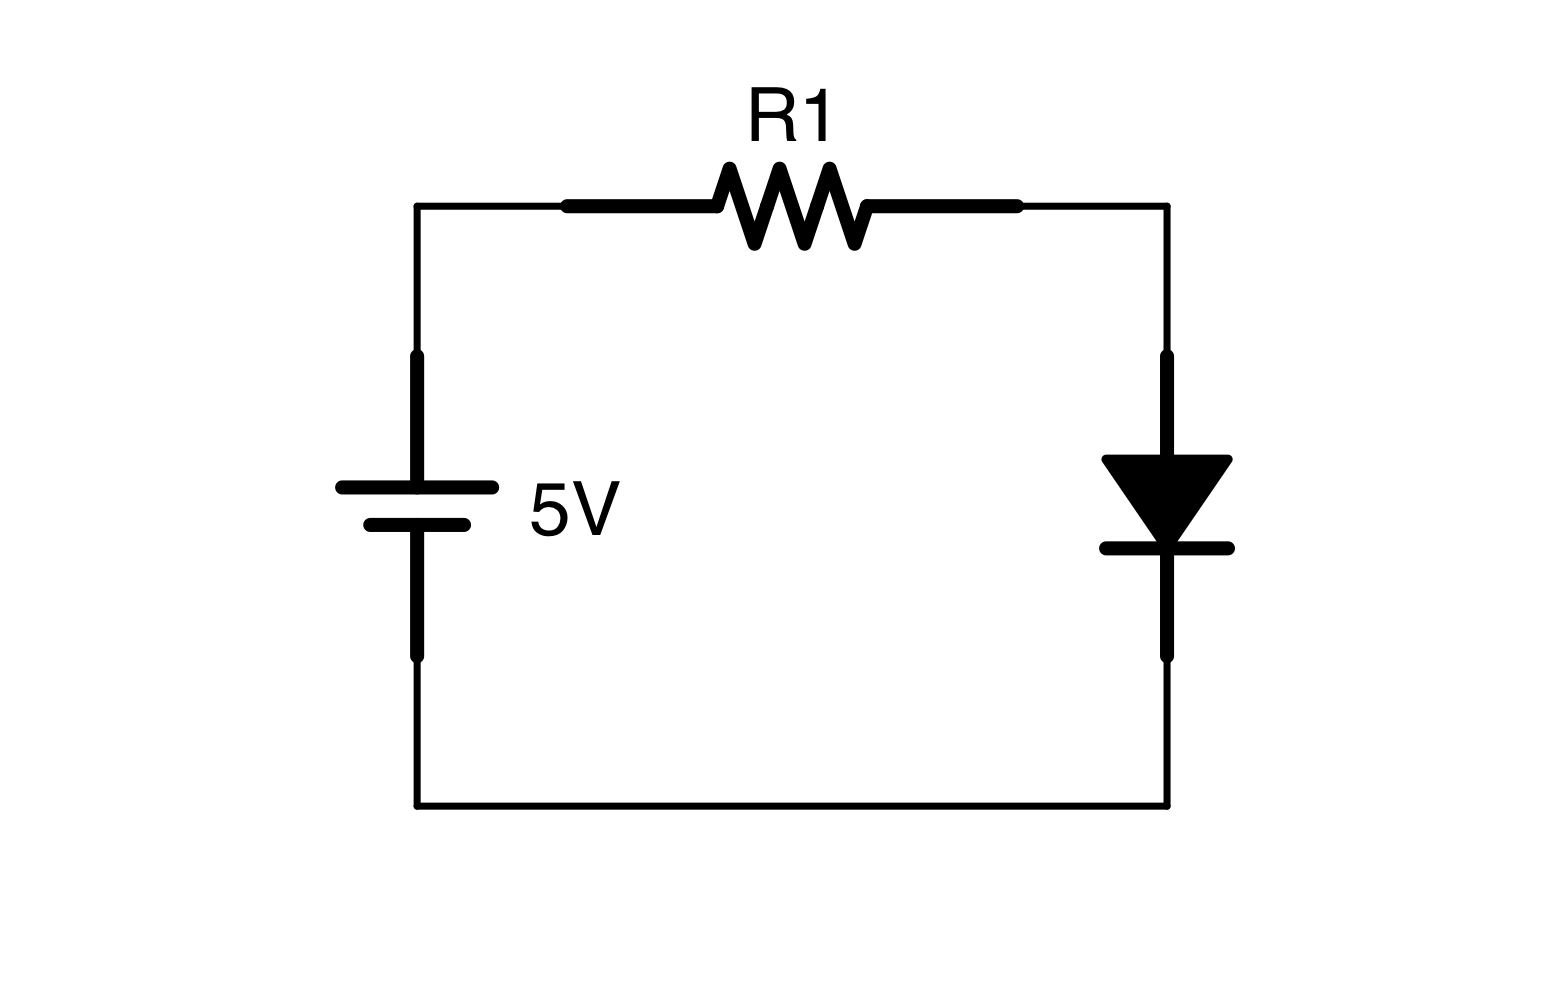
\includegraphics[scale=0.08]{DiodeApplyEx1.png}
\item Let's say instead of a standard diode, the diode is a blue LED.  Recalculate the current going through each component and the voltage drops for each component.
\item In the circuit below, calculate how much current is flowing through each component and each component's voltage drop if R1 is $300\myohm$, R2 is $400\myohm$, and R3 is $500\myohm$.  \\ 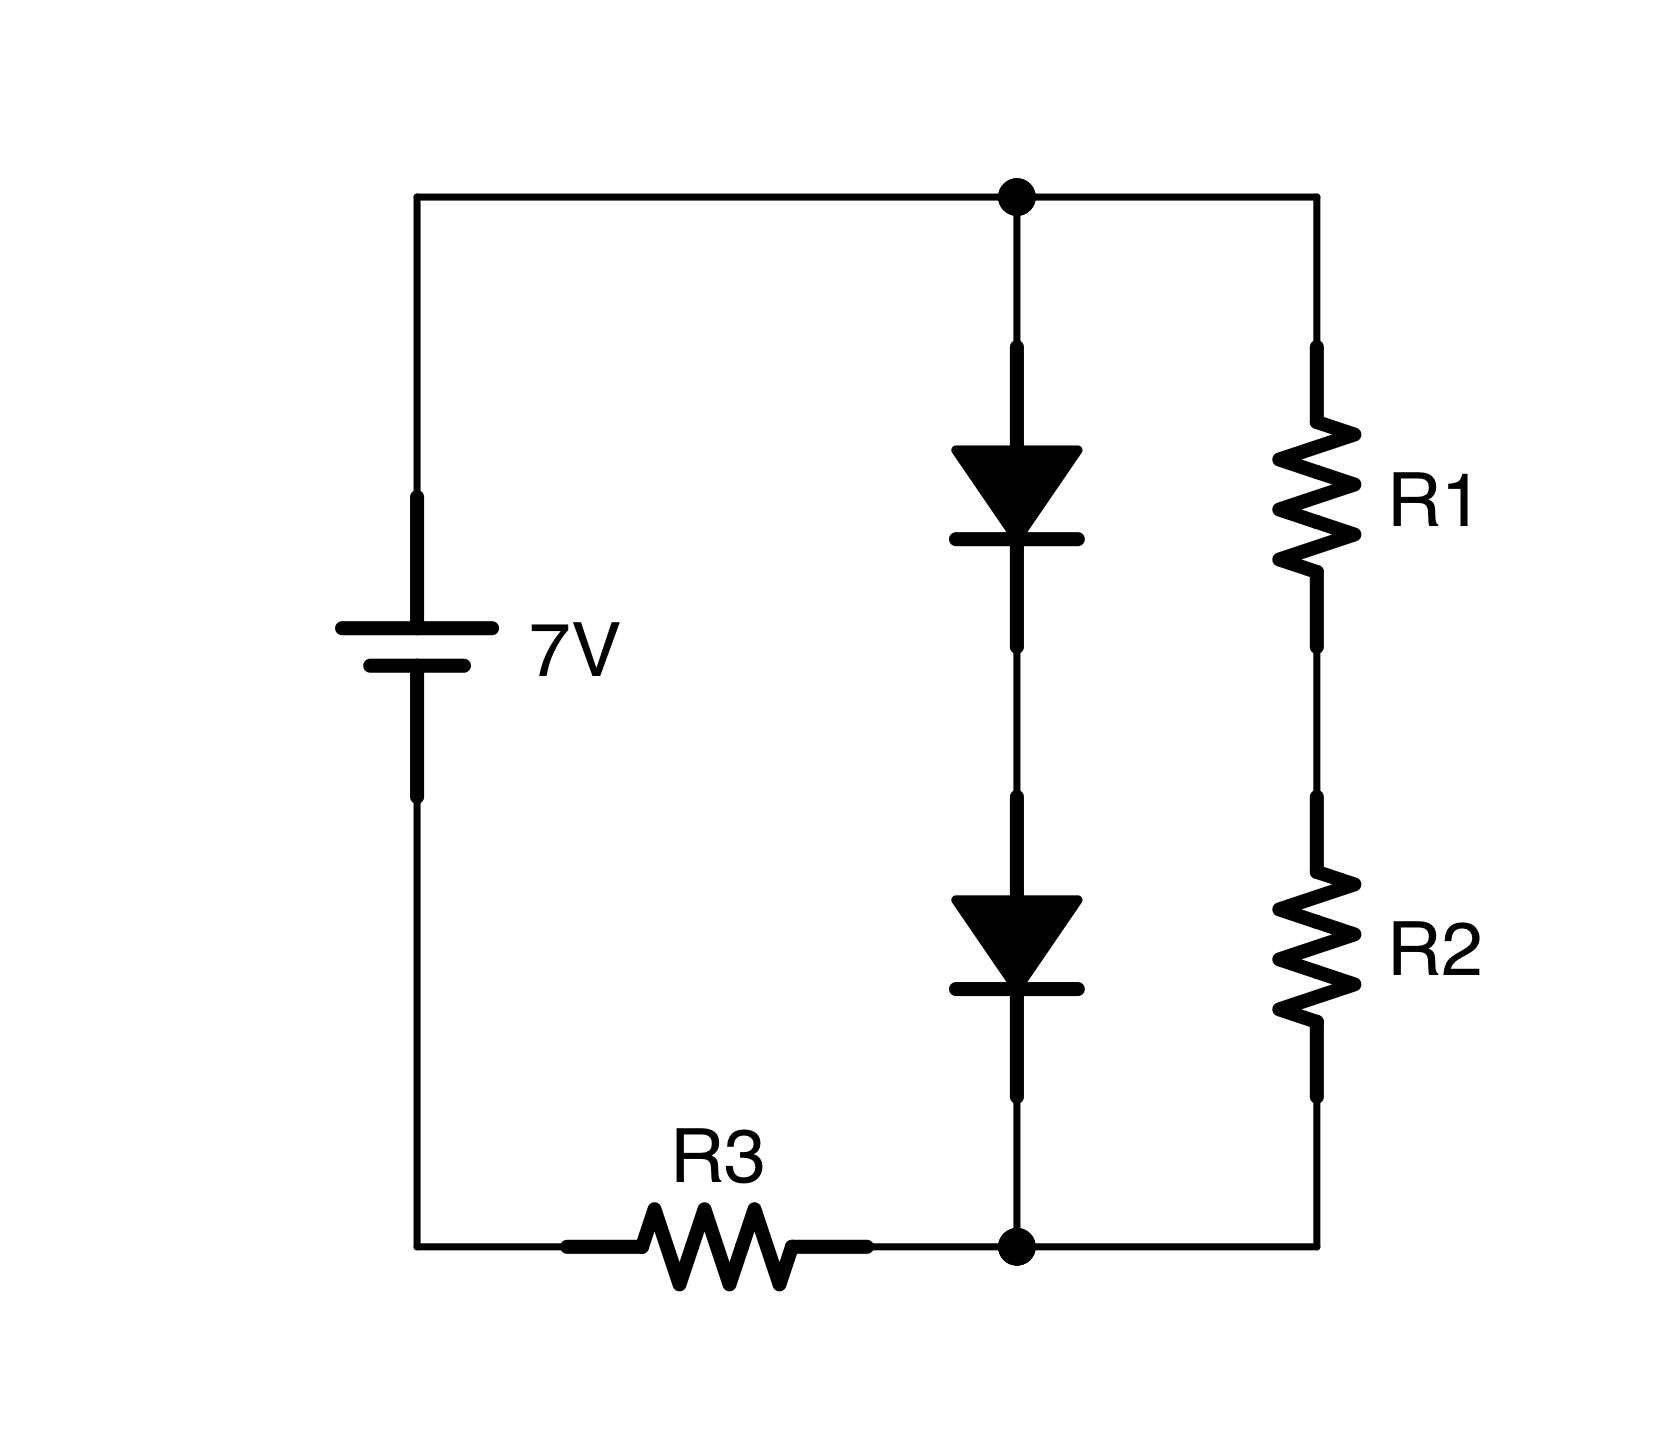
\includegraphics[scale=0.08]{DiodeApplyEx2.png}
\item Draw a circuit that provides a 6-volt regulated power supply to circuit load from a 9-volt battery using regular diodes.  Choose a resistor that works efficiently for a circuit load of $500\myohm$ and operates with a battery voltage from $7\myvolt$ to $9.6\myvolt$.  What is the current at the lowest and highest ranges of the battery?  How much is used by the circuit load and how much is wasted through the diodes in each configuration?
\item Draw an equivalent circuit to the previous question using a Zener diode instead of normal diodes.
\end{enumerate}

